\documentclass[11pt]{article}
\usepackage[margin=1in]{geometry}
\usepackage{amsmath,amssymb,amsthm}
\usepackage{tikz}
\usepackage{hyperref}
\usepackage{enumitem}
\usepackage{booktabs}

\hypersetup{colorlinks=true,linkcolor=blue!50!black,citecolor=blue!50!black,urlcolor=blue!50!black}

\newtheorem{principle}{Principle}
\newtheorem{example}{Example}

\newcommand{\dd}{\mathrm{d}}
\newcommand{\vv}[1]{\mathbf{#1}}

\title{On (Non-)Interchangeable Limits in Physics:\\
\large From a Beam on Three Pillars to the Point Electron and the Thermodynamic Limit}
\author{}
\date{\today}

\begin{document}
\maketitle

\begin{abstract}
\noindent
Physics advances largely by replacing complicated systems with idealized limits: the point particle, the rigid body, the continuum, the thermodynamic limit, the classical ($\hbar\to0$) limit. These idealizations are so routine that it is easy to forget they are genuine limiting procedures, valid only under conditions that are rarely stated. When a system depends on a single small (or large) parameter, sending that parameter to its limiting value is usually harmless. Most interesting problems, however, carry \emph{two or more} such parameters, and it is a basic fact of analysis that iterated limits need not commute: $\lim_{\varepsilon\to0}\lim_{\delta\to0} f$ can differ from $\lim_{\delta\to0}\lim_{\varepsilon\to0} f$, or the joint limit may fail to exist at all. We study this phenomenon through three worked examples: a beam resting on three rigid pillars, whose reaction forces depend on whether the beam or the pillars are idealized as rigid first; Frenkel's classical point electron, whose self-energy, electromagnetic mass, and radiation-reaction dynamics depend on the order in which the electron's radius is sent to zero and its bare mass is renormalized; and the thermodynamic limit in statistical mechanics, where spontaneous magnetization exists only if the system-size limit is taken \emph{before} the symmetry-breaking field is switched off, never the other way around. We contrast these with limits that are safe -- the same point-particle and rigid-body idealizations, used elsewhere, cause no trouble at all -- and extract a general diagnostic, rooted in the classical theory of singular perturbations, for telling in advance which limits are dangerous.
\end{abstract}

\tableofcontents

% ============================================================
\section{Introduction}
% ============================================================

Physics is, in large part, a science of controlled idealization. We compute planetary orbits by treating planets as point masses; we compute the deflection of a loaded shelf by treating steel as a rigid body; we compute the pressure of a gas by treating $N\sim10^{23}$ molecules as if $N=\infty$; we compute chemical bonding by treating nuclei as fixed classical points while treating electrons quantum mechanically; we recover ray optics from wave optics by sending the wavelength to zero. Each of these is a genuine mathematical limit -- of a size, a compliance, an inverse particle number, a wavelength -- applied to a more complete underlying theory. The success of these idealizations is one of the great practical facts of physics: point-particle celestial mechanics is accurate to many decimal places; rigid-body statics designs bridges that stand for a century; the thermodynamic limit predicts the boiling point of water.

It is worth asking \emph{why} these limits are safe, because the answer clarifies exactly when they stop being safe. A limit in a single parameter, $\varepsilon\to0$, is unproblematic whenever the quantity of interest is a continuous (indeed usually analytic) function of $\varepsilon$ near $\varepsilon=0$: the answer at small but finite $\varepsilon$ differs from the idealized answer only by a small, controllable correction, and nothing is lost by setting $\varepsilon=0$ outright. Trouble begins when a problem depends on \emph{two or more} such parameters that are idealized together. Elementary analysis already warns us that double limits need not commute, and, more importantly for physics, that the two possible iterated limits can correspond to two entirely different physical scenarios -- because the order in which we idealize encodes an assumption about which physical mechanism is responsible for resolving whatever the un-idealized, finite-parameter system needed to resolve. Get the order wrong, and the model quietly answers a different question than the one being asked.

This paper works through that idea using three case studies chosen to span mechanics, classical field theory, and statistical mechanics: a beam resting on three pillars (Section~3), Frenkel's classical point electron (Section~4), and the thermodynamic limit of a ferromagnet (Section~5). In each case a naive, single-minded idealization is either ambiguous or actively misleading, and the resolution requires tracking a second parameter -- an elastic compliance, a bare mass, a symmetry-breaking field -- through the limit alongside the first. Section~6 then explains, in the same language, why the \emph{same kind} of idealization (point particle, rigid body) is perfectly safe in other, more common uses. Section~7 distills the discussion into a short diagnostic checklist. Section~2 first sets up the necessary piece of elementary analysis.

% ============================================================
\section{The mathematics of non-commuting limits}
% ============================================================

The phenomenon at the heart of this paper already appears in single-variable calculus applied to two variables. Consider
\begin{equation}
f(x,y) = \frac{x^2}{x^2+y^2}, \qquad (x,y)\neq(0,0).
\end{equation}
For any fixed $y\neq0$,
\begin{equation}
\lim_{x\to0} f(x,y) = 0 \quad\Longrightarrow\quad \lim_{y\to0}\Big(\lim_{x\to0}f(x,y)\Big) = 0,
\end{equation}
while for any fixed $x\neq0$,
\begin{equation}
\lim_{y\to0} f(x,y) = 1 \quad\Longrightarrow\quad \lim_{x\to0}\Big(\lim_{y\to0}f(x,y)\Big) = 1.
\end{equation}
The two iterated limits disagree, and in fact the joint limit $\lim_{(x,y)\to(0,0)}f(x,y)$ does not exist at all: approaching the origin along the ray $y=\lambda x$ gives $f = 1/(1+\lambda^2)$, a different value for every slope $\lambda$. There is no way to ``just set $x=y=0$''; the answer one gets depends entirely on the \emph{path} by which the two small parameters are sent to zero together.

This is not a pathology invented for textbooks. It is the generic behavior of a two-parameter limit unless one can show, in addition to the two iterated limits agreeing, that the convergence is \emph{uniform} -- that $f(x,y)$ is close to its limiting value for \emph{all} small $(x,y)$ simultaneously, not just along special directions. Physical idealizations are exactly this kind of two-parameter limit whenever a problem carries two small (or large) quantities -- a size and a coupling, a compliance and a stiffness, an inverse system size and a symmetry-breaking field -- that are both being sent to an extreme value in the course of ``simplifying'' the problem.

The same structure reappears, in disguise, in the classical theory of \emph{singular perturbations}. Consider a boundary-value problem such as
\begin{equation}
\varepsilon\, y''(x) + y'(x) = g(x), \qquad y(0)=y_0,\ \ y(1)=y_1,
\end{equation}
with $\varepsilon>0$ small. At $\varepsilon=0$ the equation degenerates from second order to first order, and a first-order equation cannot in general satisfy \emph{two} boundary conditions. The naive limit ``set $\varepsilon=0$'' therefore does not smoothly approach the true small-$\varepsilon$ solution: instead, the true solution develops a thin \emph{boundary layer}, near one endpoint, across which $y$ changes rapidly to absorb the boundary condition that the reduced ($\varepsilon=0$) equation cannot satisfy. Away from the layer the reduced equation is an excellent approximation; inside it, it is not. The parameter $\varepsilon$ multiplies the \emph{highest derivative} in the equation, and it is precisely this feature -- a small parameter multiplying the term that carries the extra structure needed to fix an otherwise under-determined problem -- that signals a dangerous limit. All three case studies below exhibit this same signature, dressed in different physical clothing.

% ============================================================
\section{Case study I: statics of a beam on three pillars}
% ============================================================

\subsection{The indeterminacy}

Consider a straight beam of total length $2L$ resting on three supports at $x=0,\,L,\,2L$ (labelled $A$, $B$, $C$), carrying a uniform load $w$ per unit length (Figure~1).

\begin{center}
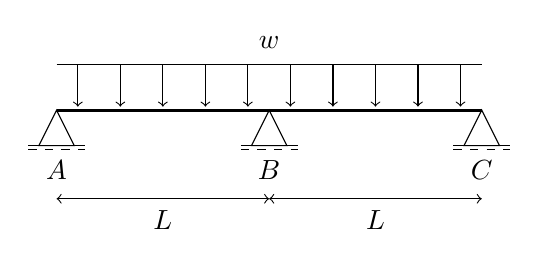
\begin{tikzpicture}[scale=0.9]
\draw[very thick] (0,0) -- (6,0);
\foreach \x in {0.3,0.9,...,5.7} { \draw[->, thin] (\x,0.65) -- (\x,0.05); }
\draw[thin] (0,0.65) -- (6,0.65);
\node at (3,0.95) {$w$};
\foreach \x/\lab in {0/A,3/B,6/C} {
  \draw (\x,0) -- (\x-0.25,-0.5) -- (\x+0.25,-0.5) -- cycle;
  \draw (\x-0.4,-0.5) -- (\x+0.4,-0.5);
  \draw[dashed] (\x-0.4,-0.55) -- (\x+0.4,-0.55);
  \node at (\x,-0.85) {$\lab$};
}
\draw[<->] (0,-1.25) -- (3,-1.25); \node at (1.5,-1.55) {$L$};
\draw[<->] (3,-1.25) -- (6,-1.25); \node at (4.5,-1.55) {$L$};
\end{tikzpicture}

\emph{Figure 1. A beam on three equally spaced supports under a uniform load.}
\end{center}

If we idealize \emph{both} the beam and the three supports as perfectly rigid, statics supplies exactly two independent equations for the three unknown reactions $R_A,R_B,R_C$:
\begin{align}
R_A+R_B+R_C &= 2wL, \label{eq:force}\\
R_A\cdot 0 + R_B\cdot L + R_C\cdot 2L &= 2wL^2. \label{eq:moment}
\end{align}
By the left--right symmetry of the problem, $R_A=R_C\equiv s$, and Eq.~\eqref{eq:moment} is then satisfied automatically by \emph{any} $s$, leaving Eq.~\eqref{eq:force} as the only real constraint: $R_B = 2wL-2s$. The rigid-body idealization thus leaves a one-parameter family of ``equilibrium'' solutions and cannot select among them. This is the textbook statement that a beam on three supports is \emph{statically indeterminate}: rigid-body statics alone has thrown away exactly the information needed to fix the answer. That information is the elastic compliance of the beam and/or the supports -- and, crucially, \emph{which} of the two is allowed to remain compliant while the other is idealized as rigid changes the answer.

\subsection{Route A: elastic beam, rigid supports}

Suppose the supports are (to excellent approximation) rigid, but the beam has finite bending stiffness $EI$. Remove the middle support and treat $R_B$ as an unknown upward force applied to the resulting simply supported beam of span $2L$. Standard beam formulas give the downward deflection at midspan due to the uniform load,
\begin{equation}
\delta_w = \frac{5w(2L)^4}{384\,EI} = \frac{5wL^4}{24\,EI},
\end{equation}
and, due to an upward point force $R_B$ at midspan,
\begin{equation}
\delta_{R_B} = \frac{R_B(2L)^3}{48\,EI} = \frac{R_B L^3}{6\,EI}.
\end{equation}
Compatibility with the rigid middle support requires zero net deflection there, $\delta_w-\delta_{R_B}=0$, giving
\begin{equation}
R_B = \frac{5wL}{4}, \qquad R_A=R_C = \frac{2wL-R_B}{2} = \frac{3wL}{8}.
\label{eq:routeA}
\end{equation}
This is the standard two-span continuous-beam result. Notice that $EI$ has cancelled out completely: the answer is finite and unique in the limit $EI\to\infty$ taken \emph{after} the compatibility equation is written down, even though setting $EI=\infty$ \emph{before} writing that equation reproduces the indeterminate mush of the previous subsection.

\subsection{Route B: rigid beam, elastic supports}

Now suppose instead that the beam is (to excellent approximation) rigid, while each support is a spring of stiffness $k$ (equal for $A,B,C$ by symmetry). A rigid beam has only two degrees of freedom: a vertical offset $y_0$ and a slope $\theta$, so $R_i = k(y_0+\theta x_i)$ for $x_i=0,L,2L$. Substituting into Eqs.~\eqref{eq:force}--\eqref{eq:moment}:
\begin{align}
3y_0+3\theta L &= \frac{2wL}{k}, \\
3y_0 L + 5\theta L^2 &= \frac{2wL^2}{k},
\end{align}
which solve to $\theta=0$ and $y_0=2wL/(3k)$, hence
\begin{equation}
R_A=R_B=R_C = \frac{2wL}{3},
\label{eq:routeB}
\end{equation}
independent of $k$. Here the redundancy is resolved not by bending but by symmetry: a perfectly rigid beam on equal, symmetric springs can only translate, so the load is shared equally among the three supports.

\subsection{The two routes disagree, and the reason why}

\begin{center}
\begin{tabular}{@{}lccc@{}}
\toprule
& $R_A$ & $R_B$ & $R_C$ \\
\midrule
Route A (elastic beam, rigid supports) & $0.375\,wL$ & $1.250\,wL$ & $0.375\,wL$ \\
Route B (rigid beam, elastic supports) & $0.667\,wL$ & $0.667\,wL$ & $0.667\,wL$ \\
\bottomrule
\end{tabular}
\end{center}

Both distributions satisfy the \emph{same} two statics equations, Eqs.~\eqref{eq:force}--\eqref{eq:moment} -- indeed they are two different points on the one-parameter family of ``equilibrium'' solutions found in Section~3.1. Which point is physically correct is decided entirely by \emph{which} compliance is allowed to survive into the limit, i.e., by the order in which ``beam rigid'' and ``supports rigid'' are imposed.

This can be made completely explicit by keeping \emph{both} compliances finite. Let the beam have stiffness $EI$ and all three supports have stiffness $k$, and define the dimensionless compliance ratio
\begin{equation}
\lambda \equiv \frac{EI}{k L^3}.
\end{equation}
Repeating the force-method calculation of Section~3.2, but now allowing the two outer supports to settle elastically as well (so that a symmetric settlement $\delta=R_A/k$ of the whole beam adds to the bending deflection relative to the chord $AC$), gives after compatibility at $B$ the closed-form result
\begin{equation}
R_B(\lambda) = wL\,\frac{24\lambda+5}{36\lambda+4}, \qquad R_A(\lambda)=R_C(\lambda)=\frac{2wL-R_B(\lambda)}{2}.
\label{eq:general}
\end{equation}
One checks directly that
\begin{equation}
\lim_{\lambda\to0} R_B(\lambda) = \frac{5wL}{4} \quad(\text{Route A}), \qquad
\lim_{\lambda\to\infty} R_B(\lambda) = \frac{2wL}{3} \quad(\text{Route B}),
\end{equation}
recovering both special cases exactly, with $R_B(\lambda)$ interpolating smoothly and monotonically between them for finite $\lambda$. Route A is the limit $k\to\infty$ at fixed $EI$ ($\lambda\to0$); Route B is the limit $EI\to\infty$ at fixed $k$ ($\lambda\to\infty$). Sending \emph{both} $EI$ and $k$ to infinity ``simultaneously,'' without specifying their ratio, is exactly as ill-posed as approaching the origin in Section~2 without specifying the slope $\lambda$: the two orders of idealization are two different rays through the same non-existent joint limit.

Physically, of course, no real beam or real support is infinitely stiff; both $EI$ and $k$ are large but finite, and $\lambda$ is simply whichever finite number the real structure has. Equation~\eqref{eq:general} shows that the rigid-body idealization is safe only once $\lambda$ has been fixed by the actual physical compliances -- exactly as the beam-equation analogy in Section~2 anticipated: $EI$ multiplies the highest (fourth) derivative in the governing beam equation $EI\,v''''=q(x)$, and letting $EI\to\infty$ before fixing $\lambda$ is precisely the singular-perturbation move of dropping the highest-derivative term before it has done its job of supplying the missing compatibility condition.

% ============================================================
\section{Case study II: Frenkel's point electron}
% ============================================================

\subsection{Self-energy and the point limit}

Model the electron classically as a charge $e$ spread over a sphere of radius $r_0$. The electrostatic self-energy is (Gaussian units)
\begin{equation}
U(r_0) = \kappa\,\frac{e^2}{r_0}, \qquad \kappa = O(1)\ \text{(e.g.\ } \kappa=\tfrac12\text{ for a thin shell, }\kappa=\tfrac35\text{ for a uniform solid sphere)},
\end{equation}
which diverges as $r_0\to0$. If this self-energy is attributed entirely to the field's inertia, one obtains an ``electromagnetic mass'' -- but the value one gets depends on \emph{how} it is computed. From the field momentum of a slowly moving charged sphere, $p_{\rm em}=\tfrac{4}{3}(U/c^2)v$, so that $p=m_{\rm em}v$ gives $m_{\rm em}^{(p)}=\tfrac{4}{3}U/c^2$; from the energy directly, $m_{\rm em}^{(E)}=U/c^2$. The mismatch by a factor of $4/3$ is the classic \emph{$4/3$ problem}: a purely electromagnetic self-energy is not, on its own, consistent with relativistic energy-momentum bookkeeping. It is resolved (Poincar\'e) by recognizing that a charge distribution held together against its own Coulomb repulsion needs a non-electromagnetic cohesive stress, and that stress's own energy and momentum supply exactly the missing $-\tfrac13$, restoring $m_{\rm total}=E_{\rm total}/c^2$. The lesson for the present paper is direct: ``send $r_0\to0$'' is not, by itself, a well-defined instruction until one has also decided how the (divergent) self-energy is to be renormalized against a second, independently divergent quantity -- here, the binding stress.

\subsection{Mass renormalization: two divergences, one limit}

The point-particle idealization becomes fully explicit, and fully double-parametered, once we ask for the electron's \emph{total} inertial mass. Write the observed mass as
\begin{equation}
m = m_0(r_0) + \frac{U(r_0)}{c^2} = m_0(r_0) + \kappa\,\frac{e^2}{r_0 c^2},
\end{equation}
where $m_0(r_0)$ is a ``bare'' mechanical mass attributed to whatever holds the charge together. The point limit $r_0\to0$ is only physically sensible if it is taken \emph{together} with $m_0(r_0)\to-\infty$ at a matched rate, $m_0(r_0) = m - \kappa e^2/(r_0c^2) + O(r_0)$, so that the finite, measured mass $m$ survives. This is nothing other than the electromagnetic prototype of mass renormalization later central to quantum field theory: a single, uncorrelated limit $r_0\to0$ is meaningless (it sends $U/c^2\to\infty$), while the \emph{correlated} double limit, in which $r_0\to0$ and $m_0\to-\infty$ are locked together so that their sum stays fixed, is perfectly well defined. Once again, the naive single-parameter idealization (``the electron is a point'') silently presupposes a highly specific joint limit in a second, hidden parameter.

\subsection{Radiation reaction: a limit that is safe for some questions and not others}

Expanding the retarded self-force on a small but finite charged sphere in powers of $r_0$ and taking $r_0\to0$ together with the mass renormalization above yields, to leading order, the Abraham--Lorentz equation of motion
\begin{equation}
m\,\dot{\vv v} = \vv F_{\rm ext} + \frac{2e^2}{3c^3}\,\ddot{\vv v},
\label{eq:AL}
\end{equation}
where $\dot{\vv v}$ is the acceleration and $\ddot{\vv v}$ its time derivative (the ``jerk''). Because it involves $\ddot{\vv v}$, Eq.~\eqref{eq:AL} is effectively a \emph{third}-order equation of motion for the position, in contrast to Newton's second-order $m\dot{\vv v}=\vv F$. This raises the order of the equation exactly as $\varepsilon\to0$ lowered the order of the boundary-layer equation in Section~2 -- here the point limit \emph{increases} the number of initial conditions needed, and the extra solutions it admits are unphysical: Eq.~\eqref{eq:AL} has runaway solutions that self-accelerate exponentially even with $\vv F_{\rm ext}=0$, and demanding that these be excluded forces the physical solutions into \emph{pre-acceleration} -- the particle begins to respond to a force an interval $\tau=2e^2/(3mc^3)$ (of order $10^{-24}\,$s for the physical electron) \emph{before} the force is applied, a mild but genuine violation of naive causality on that timescale.

Both pathologies -- runaway solutions and pre-acceleration -- are artifacts of having taken $r_0\to0$ specifically \emph{in the radiation-reaction term}, before the internal structure of the charge has had a chance to regularize the self-force at short times. Keeping $r_0$ finite removes both problems (at the cost of reintroducing internal structural dynamics that must themselves be modeled), just as keeping $EI$ or $k$ finite removed the indeterminacy of the beam. This is precisely the sense in which the point-particle limit is \emph{singular} for the specific question ``what is the self-consistent equation of motion including radiation reaction?''

It is worth emphasizing, by contrast, that the very same point limit is completely \emph{safe} for other questions about the same object: Rutherford scattering, planetary-orbit-style Coulomb dynamics, and multipole expansions of the field far from the charge all depend on $r_0$ only through smooth, subdominant corrections of relative size $(r_0/L)^n$, where $L$ is the relevant external length scale, and these corrections vanish continuously as $r_0\to0$ with no hidden second parameter involved. The point-electron idealization is thus simultaneously excellent (for scattering and orbits) and treacherous (for self-energy and radiation reaction) -- the difference is entirely about \emph{which question is being asked}, not about the idealization itself. Frenkel's own 1926 model of a relativistic, spinning point electron sits squarely in this tradition: it sidesteps the internal-structure question by fiat (endowing the point particle with an intrinsic spin and magnetic moment rather than deriving them from a charge distribution), buying calculability at the price of leaving the self-energy and radiation-reaction issues exactly where the discussion above leaves them.

% ============================================================
\section{Case study III: the thermodynamic limit and spontaneous magnetization}
% ============================================================

For a magnetic system of $N$ spins in an external field $h$ at temperature $T$, the partition function $Z_N(T,h)$ is a finite sum of exponentials of the spin configuration energies, hence an entire (analytic) function of $h$ and $T$ for every finite $N$. In particular, for $h=0$ the up--down symmetry of the Hamiltonian forces the average magnetization per spin to vanish \emph{exactly} for every finite $N$:
\begin{equation}
m(T,h=0,N) = 0 \qquad \text{for all finite } N.
\end{equation}
Yet real ferromagnets below their Curie temperature $T_c$ exhibit a nonzero \emph{spontaneous} magnetization at zero field. The resolution is again a matter of the order of two limits. Define
\begin{equation}
m_s(T) \equiv \lim_{h\to0^+}\ \lim_{N\to\infty}\ m(T,h,N).
\end{equation}
For $T<T_c$ this limit is nonzero: sending $N\to\infty$ \emph{first}, at fixed small $h>0$, allows the free-energy landscape to develop two deep, well-separated minima (``up'' and ``down''), and the infinite system, prepared with an infinitesimal field, is trapped in one of them even after the field is switched off. But the \emph{opposite} order,
\begin{equation}
\lim_{N\to\infty}\ \lim_{h\to0}\ m(T,h,N) = \lim_{N\to\infty} 0 = 0,
\end{equation}
gives identically zero at every temperature, because the inner limit is zero for every finite $N$ by the symmetry argument above. Spontaneous symmetry breaking is, in this precise sense, only ever visible in one of the two iterated limits: the thermodynamic limit must be taken \emph{before} the symmetry-breaking field is removed, never after. A closely related statement is the Lee--Yang picture of phase transitions: the zeros of $Z_N$ in the complex-field plane are, for finite $N$, always off the physical (real) axis, so that $Z_N$ and all its finite-$N$ thermodynamic functions are perfectly smooth; a genuine non-analyticity -- a true phase transition -- can only appear where those zeros pinch the real axis as $N\to\infty$. Once again, a physically essential phenomenon (ferromagnetism, phase transitions generally) is invisible unless a particular one of two possible iterated limits is used, and the finite-$N$, finite-$h$ system does not, by itself, tell you which order is the physically relevant one; that has to be supplied from outside, by the physical fact that real magnets are prepared in one broken-symmetry state at a time, not in a symmetric superposition of both.

% ============================================================
\section{Why some limits are safe}
% ============================================================

The three case studies above should not be read as an indictment of point-particle or rigid-body idealizations in general -- both are used successfully, constantly, throughout physics. What distinguishes a safe use from a dangerous one is not the idealization itself but the \emph{role} the discarded parameter was playing in the finite theory.

\begin{principle}
A limiting idealization is safe (the order of limits does not matter, and a single limit suffices) when the discarded parameter enters the quantity of interest only as a smooth, subdominant correction that vanishes continuously as the parameter is removed.
\end{principle}

This is exactly the situation in planetary mechanics (finite planetary radius enters orbital dynamics only through small, regular tidal and multipole corrections), in Rutherford-style scattering (finite nuclear size enters the cross-section as a regular form-factor correction, negligible when the probe wavelength is much larger than the nucleus), and in ordinary, \emph{statically determinate} rigid-body mechanics, where the number of unknown constraint forces already matches the number of equilibrium equations before any compliance is introduced, so elastic corrections enter as small, regular shifts rather than as the sole source of a missing equation. The thermodynamic limit is likewise safe for the overwhelming majority of bulk thermodynamic quantities -- the equation of state, the specific heat away from a critical point, the equilibrium constant of a chemical reaction -- because these depend smoothly on $1/N$ and converge to the same value regardless of how any auxiliary field is handled.

\begin{principle}
A limiting idealization is dangerous when the discarded parameter is doing one of three jobs in the finite theory: (i) resolving a redundancy or degeneracy (a statically indeterminate structure, a degenerate ground-state manifold); (ii) regularizing a formally divergent, self-referential quantity (a self-energy, a self-force); or (iii) selecting among multiple locally stable branches or vacua (spontaneous symmetry breaking, runaway versus physical solutions of an equation of motion).
\end{principle}

All three case studies above instantiate exactly one of these three roles: the beam's redundancy (i), the point electron's self-energy and self-force (ii), and the ferromagnet's broken symmetry (iii).

% ============================================================
\section{A diagnostic for dangerous limits}
% ============================================================

The discussion above suggests a short, practical checklist for deciding, in advance, whether a proposed idealization is likely to be safe.

\begin{enumerate}[label=(\arabic*)]
\item \textbf{Count the constraints.} If the idealized (e.g.\ rigid, point-like) description leaves more unknowns than equations -- a redundancy -- some discarded compliance is doing essential work, and the idealization must be taken only after that compliance has fixed the redundancy.
\item \textbf{Look for self-reference.} If the quantity of interest involves a source acting on its own field, or any other quantity that diverges as the idealization is approached, expect a second, compensating divergence (a bare mass, a counterterm, a binding stress) that must be tracked through the same limit.
\item \textbf{Look for a symmetry that would force a trivial answer.} If an exact symmetry of the un-idealized, finite system would make the naive order of limits give zero (or some other symmetric, ``un-broken'' value) by fiat, check whether the physically relevant answer instead requires the symmetry-breaking parameter to be removed only \emph{after} the idealizing limit.
\item \textbf{Check whether the discarded parameter multiplies the highest derivative} in the governing equation (as $EI$ does in the beam equation, or as the internal structure of a charge does in the retarded self-force). If so, the limit is a singular perturbation, and a boundary layer, runaway mode, or other qualitative change in the solution set should be expected.
\item \textbf{When in doubt, compute along more than one path.} If a two-(or more)-parameter idealization gives different answers along different paths to the same nominal limit (as in the toy example of Section~2), the safe procedure is to keep the physically relevant ratio of the two parameters fixed at its true, finite value, rather than sending either parameter to infinity ``first.''
\end{enumerate}

None of this is a reason to distrust idealization as a method; it is, if anything, a reason to trust it more, because it turns an occasional embarrassing paradox (a beam problem with no unique answer, an electron with infinite self-energy, a symmetric theory that somehow predicts a magnet) into a routine calculation once the second, hidden parameter is identified and tracked through the limit alongside the first.

% ============================================================
\section{Conclusion}
% ============================================================

Idealized limits are indispensable, and in the great majority of their uses they are also perfectly safe: the point particle, the rigid body, the continuum, and the thermodynamic limit each work because the physics they discard enters only as a small, smooth correction. But whenever an idealizing parameter is secretly doing double duty -- resolving a redundancy, regularizing a self-interaction, or selecting a symmetry-broken branch -- the limit becomes a genuine two-(or more-)parameter limit in the technical sense of Section~2, and the order in which the idealizations are imposed is no longer a matter of convenience but a physical assumption in its own right, one that must be justified by the actual mechanism operating in the un-idealized system. The beam on three pillars, the point electron, and the thermodynamic limit of a ferromagnet each illustrate a different flavor of this same structure -- static redundancy, field-theoretic self-reference, and spontaneous symmetry breaking, respectively -- and, not coincidentally, each historically forced the development of new formal machinery (the force method and compatibility conditions in structural mechanics; mass renormalization in classical and later quantum field theory; the Lee--Yang theory of phase transitions in statistical mechanics) precisely in order to tame it. Recognizing the common mathematical skeleton beneath these episodes -- non-commuting iterated limits, in the elementary sense of Section~2 -- is a useful piece of general-purpose intuition for noticing, before the paradox appears, when an idealization needs a second parameter kept on a leash.

% ============================================================
\begin{thebibliography}{99}

\bibitem{Jackson} J. D. Jackson, \emph{Classical Electrodynamics}, 3rd ed. (Wiley, New York, 1998), Ch.~16.

\bibitem{Rohrlich} F. Rohrlich, \emph{Classical Charged Particles}, 3rd ed. (World Scientific, Singapore, 2007).

\bibitem{Dirac1938} P. A. M. Dirac, ``Classical theory of radiating electrons,'' Proc. R. Soc. Lond. A \textbf{167}, 148 (1938).

\bibitem{Timoshenko} S. Timoshenko and J. M. Gere, \emph{Mechanics of Materials} (Van Nostrand Reinhold, New York, 1972), chapters on statically indeterminate beams.

\bibitem{LandauLifshitz} L. D. Landau and E. M. Lifshitz, \emph{Statistical Physics}, Part 1, 3rd ed. (Pergamon, Oxford, 1980).

\bibitem{LeeYang} T. D. Lee and C. N. Yang, ``Statistical theory of equations of state and phase transitions. II. Lattice gas and Ising model,'' Phys. Rev. \textbf{87}, 410 (1952).

\bibitem{Goldenfeld} N. Goldenfeld, \emph{Lectures on Phase Transitions and the Renormalization Group} (Addison-Wesley, Reading, MA, 1992).

\bibitem{BenderOrszag} C. M. Bender and S. A. Orszag, \emph{Advanced Mathematical Methods for Scientists and Engineers} (McGraw-Hill, New York, 1978), chapters on singular perturbation theory and boundary layers.

\end{thebibliography}

\end{document}
